%% =====================================================================
%%  DRAFT — ACM two-column (sigconf), anonymous review mode
%%  Kamer: archive-grounded generative-agent sandbox of Dutch parliament
%%  S1/S2/S3 numbers from runs/kamer/s1.json and runs/kamer/paper_exps.json.
%% =====================================================================
\documentclass[sigconf,review,anonymous]{acmart}

\usepackage{booktabs}
\usepackage{multirow}
\usepackage{subcaption}
\usepackage{enumitem}
\usepackage{algorithm}
\usepackage{algpseudocode}
\usepackage{tikz}
\usetikzlibrary{positioning,arrows.meta,fit,backgrounds,shapes.geometric}

\newcommand{\tbd}[1]{\textcolor{red}{#1}}
\newcommand{\note}[1]{\textcolor{blue}{[\textbf{Note:} #1]}}
\newcommand{\sys}{\textsc{Kamer}}
\newcommand{\figph}[2]{%
  \fbox{\parbox[c][#2][c]{0.95\linewidth}{\centering\small\textcolor{red}{#1}}}}

\setcopyright{acmlicensed}
\copyrightyear{2027}
\acmYear{2027}
\acmDOI{XXXXXXX.XXXXXXX}
\acmConference[WWW '27]{The ACM Web Conference 2027}{2027}{City, Country}
\acmISBN{978-1-4503-XXXX-X/2027/06}

\begin{document}

\title[Countering Present-Day Bias in LLM Agents]{Countering Present-Day
Bias in LLM Agents: An Archive-Grounded Simulation of the Nineteenth-Century
Dutch Parliament}

\author{Anonymous Author(s)}
\affiliation{%
  \institution{Anonymous Institution}
  \city{City}
  \country{Country}}
\email{anonymous@example.com}

\renewcommand{\shortauthors}{Anonymous et al.}

%% =====================================================================
\begin{abstract}
LLM agents increasingly simulate societies, but they carry present-day
bias. Placed in a nineteenth-century parliament, they can use
twenty-first-century policy language and refuse the period's adversarial
register. Generative-agent sandboxes such as Smallville (Park
et al., 2023) do not correct this: any agent may speak anywhere, and present-day
readers judge believability. We present \sys{}, a
sandbox of the Dutch parliament that moves historical constraints out of
the language model and into the world. Agents are seeded from attested
speakers in the 1814--1899 proceedings, conditioned on period debate, and
filtered for anachronism. A \emph{role automaton} and the standing orders
decide who may act: only a recognised member may speak, and journalists
may watch from the press gallery but never take the floor. An in-world
stenographer writes a \emph{simulated Handelingen} of recognised floor
speech, comparable with the real, selective record. No
modern vocabulary entered the simulated record, and a historian judged
\sys{}'s interview answers more plausible for a late-1890s member than
those of a Smallville-like baseline (17 wins, 8 losses, 11 ties). A
resignation rumour reached almost all members yet appeared in only $4\%$
of the record. Like the real Handelingen, the simulated record contains no
speech by journalists; without the floor rules, journalists produce
$4.3\%$ of it, and swapping the heuristic planner for \texttt{gpt-4o-mini}
changes neither result. Present-day bias, these results suggest, is
better countered by archives and institutions than by prompts.
And because procedure alone separates what parliament knew from what it
recorded, silence in the Handelingen cannot by itself be read as
ignorance.
\end{abstract}

\begin{CCSXML}
<ccs2012>
<concept>
<concept_id>10010147.10010341.10010349.10011810</concept_id>
<concept_desc>Computing methodologies~Multi-agent systems</concept_desc>
<concept_significance>500</concept_significance>
</concept>
<concept>
<concept_id>10010405.10010469</concept_id>
<concept_desc>Applied computing~Arts and humanities</concept_desc>
<concept_significance>500</concept_significance>
</concept>
<concept>
<concept_id>10003120.10003121</concept_id>
<concept_desc>Human-centered computing~Human computer interaction (HCI)</concept_desc>
<concept_significance>300</concept_significance>
</concept>
</ccs2012>
\end{CCSXML}

\ccsdesc[500]{Computing methodologies~Multi-agent systems}
\ccsdesc[500]{Applied computing~Arts and humanities}
\ccsdesc[300]{Human-centered computing~Human computer interaction (HCI)}

\keywords{generative agents, sandbox simulation, large language models,
digital history, parliamentary proceedings, computational social science}

\begin{teaserfigure}
  \centering
  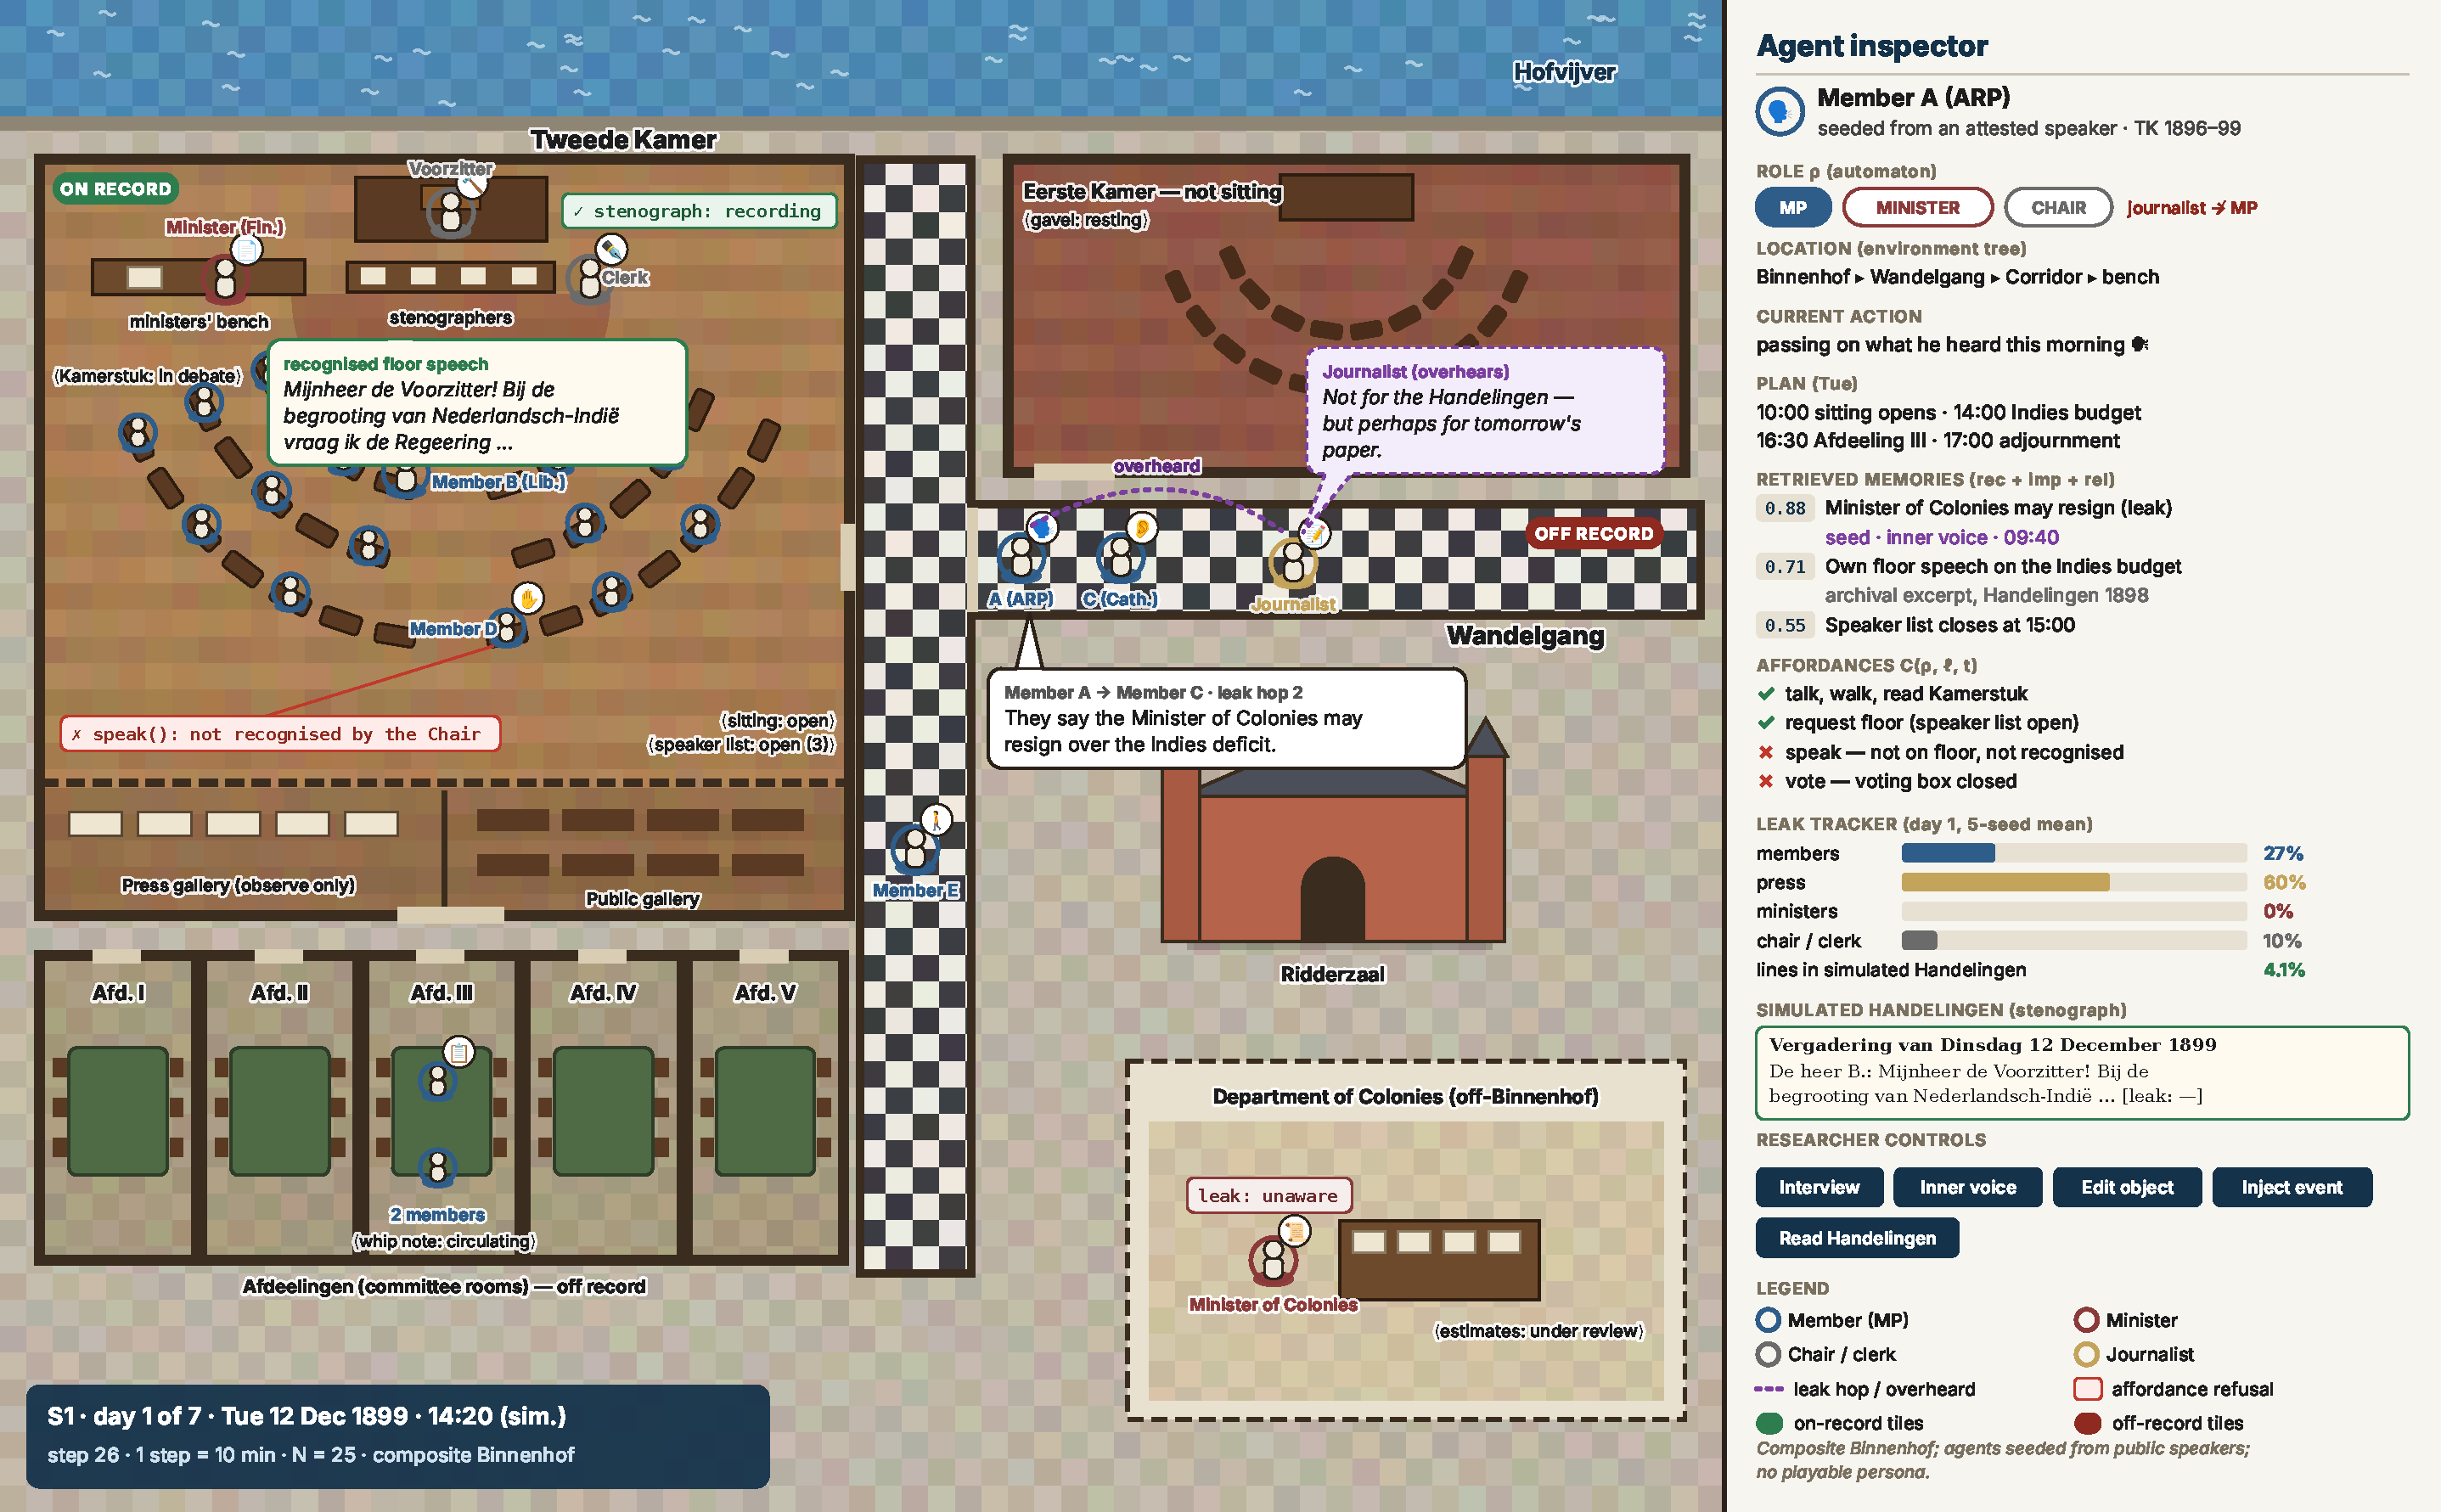
\includegraphics[width=\textwidth]{figure/kamer_sandbox.pdf}
  \caption{The \sys{} sandbox on day~1 of S1, our simulated one-week sitting
  of December 1899 (composite Binnenhof; agents seeded from public speakers,
  $N{=}25$). In the Tweede Kamer, a recognised member
  speaks on the East Indies budget while an unrecognised member is refused
  the floor. In the wandelgang, Member~A tells Member~C that the Minister of
  Colonies may resign (rumour hop~2); a journalist overhears, but the leak
  does not enter the Handelingen. The minister, in the Department of Colonies,
  remains unaware. Right: the inspector shows the agent's role, its location
  in the environment tree, standing-order affordances, retrieved memories,
  the S1 leak tracker, and researcher controls. No persona is playable.}
  \Description{A top-down map of a composite Binnenhof with the Tweede Kamer
  floor, wandelgang, committee rooms, press gallery and an agent inspector.}
  \label{fig:teaser}
\end{teaserfigure}

\maketitle

%% =====================================================================
\section{Introduction}
\label{sec:intro}

Historians reason about processes they cannot observe. How a rumour
travelled through a legislature, why one sitting ended in a cabinet crisis
and another in silence, what members knew but never said: these are
questions about mechanisms, yet the surviving sources record outcomes, and
they record them selectively. Counterfactual questions are harder still,
since no archive shows what would have happened had the Chair been
stricter or a rumour reached the minister a day earlier. Simulation makes
such reasoning explicit. By modelling the actors of a period and the rules
they followed, a historian can test whether a hypothesised mechanism
suffices to produce the patterns in the archive, and can explore
alternatives that the record cannot show~\cite{epstein2006generative}.
Agent-based models have been used in this way for settlement and
population history~\cite{axtell2002population}, but their hand-crafted
rules cannot represent debate, the medium through which much of political
history unfolded.

Generative agents~\cite{park2023generative} remove this limitation. In
Smallville, 25 agents driven by large language models (LLMs) live in a
tile-based sandbox town. Each agent perceives its surroundings, stores
observations in a memory stream, synthesises reflections, and makes plans;
together, the agents produce emergent social behaviour such as information
diffusion, relationship formation, and the coordination of a Valentine's
Day party. Because the world is an interactive sandbox, a user can watch
agents move, read their dialogue, interview them, and intervene. Later
work has scaled such agent societies to more than a thousand
agents~\cite{al2024projectsid,piao2025agentsociety}. Agents that talk make
it possible to simulate deliberative institutions in their own words.

A parliament is a natural place to begin, because its deliberation is
unusually well recorded. For the Netherlands, the \emph{Handelingen der
Staten-Generaal} cover every sitting of the States General from the
restoration of 1814 to the present; they have been digitised by
Staten-Generaal Digitaal and published on the Web as PoliticalMashup XML
under CC0~\cite{marx2012dutchparl,marx2010dutchparl}. Historians use this
record to study parties, cabinets, colonial policy, and the evolution of
parliamentary language. Yet the Handelingen are not a complete transcript
of political life. They are an \emph{official} record: produced under
standing orders, edited, and silent about the corridor.

Applying generative agents to such a parliament exposes three problems.
First, the language model carries \emph{present-day bias}, which
historians call presentism. Trained largely on contemporary Web text, LLM
backbones make simulated members speak twenty-first-century policy
language, refuse the adversarial register of nineteenth-century
debate~\cite{wang2025identity,bender2021parrots}, or describe themselves
as English-style ``MPs'' rather than members of a particular chamber; a
persona prompt alone offers no guarantee against this bias. Second, the
sandbox world is \emph{ungated}: any agent may walk anywhere and speak to
anyone, so nothing prevents a journalist from taking the floor or a member
from interrupting the Chair, and procedure is left to the model's
willingness to role-play. Third, existing sandboxes are validated against
\emph{present-day} judgements of believability, whereas a historical
simulation must be checked against an archive that is itself a selective
instrument: the Handelingen record the floor, not the wandelgang (the
lobby corridor).

We address these problems by moving historical constraints out of the
language model and into the world, where they can be inspected and
tested. The archive supplies who may appear and how they spoke: agents
are seeded from attested speakers, prompts are conditioned on period
proceedings, and an anachronism filter regenerates utterances foreign to
the simulated year. Institutions decide who may act: a role automaton and
the standing orders gate every action, so a journalist cannot take the
floor however the model is prompted. The archive's own selection becomes
the validation target: an in-world stenographer writes only recognised
floor speech, producing a simulated record that can be compared with the
real one.

We implement this design in \sys{}, an archive-grounded generative agent
sandbox of the nineteenth-century Dutch parliament. \sys{} is instantiated
on a composite Binnenhof, the parliamentary complex in The Hague, and
seeded from the 1814--1899 slice of the PoliticalMashup corpus
(Figure~\ref{fig:teaser}). As in Smallville, the world is a 2D map backed
by an environment tree of areas and stateful objects; unlike Smallville,
every edge of that tree is gated by \emph{institutions}: the agent's role
(Chair, member, minister, clerk, journalist), the Reglement van Orde (the
standing orders), and whether the sitting is open. Corridor talk travels
with provenance and distortion but reaches the simulated Handelingen only
when a recognised speaker raises it on the floor. Historians use the
sandbox interactively: they inspect and interview agents, edit object
states (``the speaker list is closed''), and inject events such as a
cabinet crisis or the 1848 constitutional revision.

Experiments with \sys{} support this design. On present-day bias, no
modern vocabulary entered the simulated Handelingen under either backend,
and a historian judged \sys{}'s interview answers more plausible for a
late-1890s member than those of a Smallville-style baseline (17 wins,
8 losses, 11 ties). Institutional outcomes, in turn, did not depend on the
backbone. Like the real Handelingen, the simulated record contains no
speech by journalists; without the floor rules, journalists produce
$4.3\%$ of it, and replacing the heuristic planner with
\texttt{gpt-4o-mini} changes neither figure. Finally, the record diverged
sharply from what parliament knew: a resignation rumour reached almost all
members within a week but appeared in only $4\%$ of the simulated record,
and doubling the Chair's strictness removed it altogether
(\S\ref{sec:results}). These results suggest that present-day bias is
better countered by archives and institutions than by prompts, and that
silence in the Handelingen cannot by itself be read as ignorance.

\sys{} does not simulate enslaved people, private households, or colonised
subjects as agents. An earlier design would have done so; historians we
consulted judged it ethically unacceptable (\S\ref{sec:ethics}). The agents
of \sys{} are public office-holders acting in public, whose words are
already on the record.

In summary, we make the following contributions:
\begin{itemize}[leftmargin=*,nosep]
  \item \textbf{Countering present-day bias outside the language model.} A design
  that places historical constraints in the archive and in institutions
  rather than in the prompt: attested personas, archival retrieval, an
  anachronism filter, and procedural gating that holds regardless of the
  backbone (\S\ref{sec:pipeline}--\S\ref{sec:agents}).
  \item \textbf{A role-constrained sandbox.} An interactive tile world of
  the Binnenhof whose environment tree, object states, and affordances encode
  the standing orders, including the split between the Tweede Kamer (lower
  house) and the Eerste Kamer (upper house), together with a parliamentary
  role automaton (\S\ref{sec:sandbox}, \S\ref{sec:agents}).
  \item \textbf{An archive-to-sandbox pipeline.} We build the world, its
  rules, and a population of attested public speakers from PoliticalMashup
  XML (8{,}745 sittings and 138{,}214 speeches in the 1814--1899 slice)
  (\S\ref{sec:pipeline}).
  \item \textbf{A simulated Handelingen and selection-aware calibration.} An
  in-world stenographer records only recognised floor speech, so that the
  simulation can be calibrated against \emph{what the archive could have
  recorded} (\S\ref{sec:calibration}).
  \item \textbf{Evaluation.} Three experiments: a simulated one-week
  sitting in December 1899 (S1), with corridor-versus-floor leak diffusion,
  ablations of the standing orders and the rumour network, and a backbone
  check with \texttt{gpt-4o-mini}; a selection-aware comparison with
  held-out Handelingen from 1890--1899 (S2); and an intervention on Chair
  strictness (S3). We also audit modern vocabulary and report a historian's
  ranking of agent interviews (\S\ref{sec:experiments}--\S\ref{sec:results}).
\end{itemize}

%% =====================================================================
\section{Related Work}
\label{sec:related}

\paragraph{Generative agents and sandboxes.} Generative
Agents~\cite{park2023generative} introduced a memory stream with retrieval
by recency, importance, and relevance, together with periodic reflection and
recursive planning, and situated 25 agents in Smallville. Open-source
reimplementations package this loop as a simulation server with a
dashboard~\cite{smallvillerepo}, and Project Sid~\cite{al2024projectsid} and
AgentSociety~\cite{piao2025agentsociety} scale the pattern to larger
populations. Related work uses LLMs as simulated survey
respondents~\cite{argyle2023outofone,aher2023turing}, economic
actors~\cite{horton2023homosilicus}, and social-network
users~\cite{gao2023s3,tornberg2023simulating}. \sys{} adopts the sandbox
and cognitive loop of Generative Agents~\cite{park2023generative}, but its
world is defined by parliamentary procedure and it is validated against an
official record.

\paragraph{Agent-based social simulation.} Classical agent-based models
(ABMs) explain macro phenomena from local
rules~\cite{schelling1971dynamic,epstein1996growing}; the generative
standard requires that a candidate explanation actually grow the
phenomenon~\cite{epstein2006generative}. Historical ABMs, notably of
Ancestral Pueblo settlement~\cite{axtell2002population}, rely on
hand-crafted rules that cannot represent debate. \sys{} follows the
generative standard: its claims concern which institutional rules suffice
to produce the patterns in the record (\S\ref{sec:discussion}).

\paragraph{Limits of LLM simulacra.} LLMs flatten identity
groups~\cite{wang2025identity}, encode representational
harms~\cite{bender2021parrots}, and may produce convincing but unfounded
behaviour~\cite{ziems2024css}. In a parliament, these failures appear as
anachronistic vocabulary, sanitised conflict, and members who
``cooperate'' instead of opposing. We audit for them explicitly
(\S\ref{sec:results}).

\paragraph{Computational parliamentary corpora.} DutchParl and
PoliticalMashup encode the Handelingen as proceedings XML with speaker,
role, party, and house metadata~\cite{marx2010dutchparl,marx2012dutchparl}.
The source scans come from Staten-Generaal Digitaal (Koninklijke
Bibliotheek), and the dataset is released under CC0 (\S\ref{sec:ethics}).
NLP on historical proceedings must cope with OCR noise and spelling
variation~\cite{ehrmann2023ner}. \sys{} uses the corpus both as a
\emph{seed} (personas, speech style, sitting calendars) and as a
\emph{calibration target} (who spoke, for how long, on which topics, and in
which house).

\paragraph{Archives as selection.} Official records are not transparent
windows onto events~\cite{trouillot1995silencing}. The Handelingen omit
what the Chair did not recognise and what members chose not to say on the
floor. \sys{} treats that selection as a design constraint: the sandbox
generates hypotheses about \emph{processes}, including the process that
produced the record, and never offers testimony about unrecorded inner
lives.

%% =====================================================================
\section{The \sys{} Sandbox}
\label{sec:sandbox}

\subsection{World: tile map and environment tree}

The world is a 2D tile map of a composite Binnenhof
(Figure~\ref{fig:teaser}). Its layout and institutions are calibrated to
the late-nineteenth-century Staten-Generaal, but it reproduces no single
historical floor plan. Following Smallville~\cite{park2023generative}, the
map is backed by an \emph{environment tree}
\[
\mathcal{T}:\ \textsf{Binnenhof}\ \triangleright\ \textsf{Area}\ \triangleright\
\textsf{Subarea}\ \triangleright\ \textsf{Object},
\]
e.g.,\\ \textsf{Binnenhof\,$\triangleright$\,Tweede Kamer\,$\triangleright$\,Right benches\,$\triangleright$\,kamerstuk}
or
\textsf{Binnenhof\,$\triangleright$\,Wandelgang\,$\triangleright$\,Corridor}.
The root node, Binnenhof, represents the whole world; its children are
areas, their children are subareas, and the leaves are objects. The areas
are the Tweede Kamer (chair's dais, stenographers' table,
griffier's (clerk's) desk, ministers' bench, left and right benches, aisle,
tribune), the Eerste Kamer (its own chair, floor, and benches), the
wandelgang, committee rooms (afdeelingen), the press gallery, and ministers'
rooms. Each tile carries an \emph{on-record} or \emph{off-record} tag,
which determines whether the stenographer may write, and a house tag
(\texttt{commons} or \texttt{senate}).

\paragraph{Two chambers.} The Staten-Generaal has been bicameral since 1815.
The Tweede Kamer is directly elected, conducts day-to-day politics, amends
and initiates bills, and is where cabinets stand or fall. The Eerste Kamer
is elected indirectly by the Provinciale Staten, sits far less often, and
may only accept or reject bills: it has no right of amendment or
initiative~\cite{pdc2024kamers}. Between 1888 and 1918, a period that
includes S1, our simulated week of Tweede Kamer sittings in December 1899
(\S\ref{sec:experiments}), the Eerste Kamer several times blocked cabinets
that held a Tweede Kamer majority. \sys{} therefore treats house membership as
an institutional attribute rather than a label. A Kamerlid of the Tweede
Kamer has no floor rights in the Eerste Kamer; ministers, who appear in
both houses, do; and \texttt{move\_amendment} is undefined on senate tiles.
Although S1 is a Tweede Kamer week, the Eerste Kamer is present on the map
and in the affordance layer, so that ``lid der Staten-Generaal'' (member of
the States General) is never an admissible self-description.

\paragraph{Stateful objects.} Every leaf of $\mathcal{T}$ is an object with
a natural-language state that agents perceive and actions change
(Table~\ref{tab:objects}). Objects make procedure concrete: the speaker list
is open or closed, the gavel opens and adjourns the sitting, the stenograph
is idle or recording, and a Kamerstuk (parliamentary paper) moves from
tabled to in debate to voted.

\begin{table}[t]
\caption{Representative sandbox objects and their states.}
\label{tab:objects}
\centering\small
\setlength{\tabcolsep}{3pt}
\begin{tabular}{lll}
\toprule
Object & States & Changed by \\
\midrule
Gavel & resting, opening, adjourned & chair \\
Speaker list & empty, open, closed & chair, griffier \\
Kamerstuk & tabled, in debate, voted, withdrawn & government, chair \\
Stenograph & idle, recording, paused & stenographer \\
Voting box & closed, open, counted & chair, griffier \\
Press-gallery desk & empty, occupied & journalist \\
Whip note & none, circulating, spent & members \\
\bottomrule
\end{tabular}
\end{table}

\subsection{Time, engine, and interface}

One simulation step corresponds to $10$ minutes of in-world time.
Sittings open on weekdays at 10:00 and adjourn at 17:00, matching the
rhythm of the Handelingen. \sys{} follows the server--client design of
open-source Smallville implementations~\cite{smallvillerepo}: a simulation
server holds the environment tree, object states, and agent memories,
advances the world with an \texttt{updateState} call, and exposes this
state over a REST API. The interface renders each agent's current action as
a short natural-language statement with an emoji. Role is shown only by a
ring colour; sprites are deliberately neutral tokens.

\subsection{Researcher interaction}

The sandbox supports five forms of interaction, all of which are logged:
\begin{itemize}[leftmargin=*,nosep]
\item \textbf{Inspect}: view an agent's role, location path, plan,
retrieved memories, affordances, and known map (Fig.~\ref{fig:teaser}, right).
\item \textbf{Interview}: pause the world and pose questions, which the
agent answers from memory without writing the exchange back
(\S\ref{sec:eval-interview}).
\item \textbf{Inner voice}: add a memory such as ``You heard in the
wandelgang that the minister will resign'', for controlled information
interventions.
\item \textbf{Edit object}: change an object state, e.g., close the speaker list.
\item \textbf{Inject event}: introduce a cabinet crisis, a closed sitting,
or the 1848 constitutional revision.
\end{itemize}
Researchers cannot ``play'' an agent: no persona can be controlled in the
first person.

%% =====================================================================
\section{Archive-to-Sandbox Pipeline}
\label{sec:pipeline}

\paragraph{Sources.} We use the non-semanticized PoliticalMashup release of
the Dutch parliamentary proceedings~\cite{marx2012dutchparl}: one XML
document per sitting from 1814 to April 2012, released under CC0. Our
working slice covers \textbf{1814--1899}: 8{,}745 sittings, of which
6{,}340 are Tweede Kamer sittings (\texttt{pm:house="commons"}), 2{,}036
are Eerste Kamer sittings (\texttt{senate}), and 369 are early or
unlabelled meetings. Of these, 7{,}348 files contain at least one
\texttt{speech} element, yielding \textbf{138{,}214} speaker-attributed
speeches. PoliticalMashup records 852 distinct \texttt{pm:member-ref}
identifiers; raw \texttt{pm:speaker} strings are far more numerous because
of OCR variation. Role attributes on speech elements are dominated by
\texttt{mp}, followed by \texttt{government} and \texttt{chair}. Party
references in the later nineteenth century include liberals,
conservatives, anti-revolutionaries, Catholics, and, by the 1890s, the
SDAP. The full corpus of Marx et al.\ continues to 2012; we leave the
post-1899 portion to future work.

\begin{table}[t]
\caption{Working slice of DutchParl (1814--1899) used to seed \sys{}.}
\label{tab:corpus}
\centering\small
\begin{tabular}{lrrr}
\toprule
 & Sittings & Speeches & Years \\
\midrule
Tweede Kamer (commons) & 6{,}340 & --- & 1814--1899 \\
Eerste Kamer (senate) & 2{,}036 & --- & --- \\
Other / early Staten-Generaal & 369 & --- & --- \\
\midrule
All sittings in slice & 8{,}745 & 138{,}214 & 86 years \\
\quad with $\geq$1 \texttt{speech} & 7{,}348 & 138{,}214 & --- \\
Member identifiers & 852 & --- & --- \\
S1 roster (TK 1896--99 sample) & 80 sittings & --- & 205 speakers \\
Holdout TK 1890--1899 (S2) & 731 & 20{,}166 & --- \\
Calibration TK 1860--1889 (S2) & 2{,}821 & 72{,}112 & --- \\
\bottomrule
\end{tabular}
\end{table}

\paragraph{Event extraction.} A schema-constrained parser reads each
sitting's Dublin Core header (date, title, house, legislative period) and
every \texttt{speech} element (speaker, role, function, party, member-ref,
text). OCR noise is retained as a property of the archive: unless a
member-ref is present, personas inherit the \emph{documented} name string
rather than a cleaned modern spelling. Every field keeps its source
attribution.

\paragraph{From records to world.} Historians translate the Reglement van
Orde and secondary literature on the Staten-Generaal into
(i)~affordance rules (who may speak, recognise, vote, or sit in the
gallery), (ii)~object schedules (sitting hours, speaker lists, budget
debates), and (iii)~the layout of $\mathcal{T}$ (6 areas, 15 subareas, and
7 objects in the S1 Binnenhof).

\paragraph{Population.} S1 samples $N{=}25$ agents from attested speakers
in Tweede Kamer sittings of 1896--1899, filtered to the offices held in
December 1899: Gleichman as Chair, Cremer and Goeman Borgesius as
ministers of the Pierson cabinet, Arntzenius as griffier, one journalist,
and 20 members. Each agent is seeded with a short persona and up to three
excerpts of the person's actual public speech. The agent for Abraham
Kuyper, leader of the Anti-Revolutionary Party, receives the persona below
and, among its excerpts, the passage that follows it, taken from the
sitting of 20 November 1896 with OCR errors preserved:
\begin{quote}\small\ttfamily\raggedright
De heer Kuyper is Kamerlid der Tweede Kamer (1899-1900). Partij: nl.p.arp.
Het publieke woord, zoo het op de vloer klinkt, is tot den Voorzitter
gericht.\par\smallskip
Mynhee r de Voorzitter! Aa n de koffie en het djatihout besteedde de Kamer
een niet onbelangrijk deel van den beschikbaren parlementairen tijd. E n
ongetwijfeld zyn ook die materieele belangen van gewicht [\ldots]
\end{quote}
(``Mr Kuyper is a member of the Tweede Kamer (1899--1900). Party:
Anti-Revolutionary. Public speech, as it sounds on the floor, is addressed
to the Chair.'' ``Mr Chairman! The Chamber spent no small part of the
available parliamentary time on coffee and teak. And these material
interests are no doubt also of weight [\ldots]'') Unlike the Smallville
seed descriptions, which cover occupation, family, and relationships, the
seed holds only public office, house, party, and attested speech; no
private life is instantiated. The persona is prepended to every LLM
prompt, and the opening of the first excerpt is reused verbatim when the
agent speaks on the floor without an LLM completion. Agents identify as
Kamerlid, minister, or Voorzitter (Chair) \emph{der Tweede Kamer} (or
Eerste Kamer), never as an English ``MP'' of an undifferentiated
Staten-Generaal. The journalist is the only role not drawn from a
\texttt{speech} element: the Handelingen do not record the press gallery,
which is precisely why the sandbox includes this role. The griffier is a
named office-holder (Arntzenius, in office 1888--1920); the stenographer is
a separate role, implemented as the observation model $O_\phi$. A
parliamentary historian reviewed
the roster, the OCR speaker cards, and the standing-order scheme
(\S\ref{sec:eval-interview}).

%% =====================================================================
\section{Role-Constrained Generative Agents}
\label{sec:agents}

\paragraph{Memory, reflection, planning.} Each agent keeps a memory stream
of observations, dialogue, and reflections. Given a query $q$, each memory
$m$ is scored by
\begin{equation}
s(m\,|\,q)=\alpha_{\text{rec}}\,\text{rec}(m)+\alpha_{\text{imp}}\,\text{imp}(m)+\alpha_{\text{rel}}\,\cos(e_m,e_q),
\label{eq:retrieval}
\end{equation}
which combines exponentially decaying recency, LLM-rated importance on a
1--10 scale, and embedding relevance, each min--max
normalised~\cite{park2023generative}. A reflection is triggered when the
summed importance of recent memories exceeds a threshold $\tau$. Plans are
produced top-down and constrained by \emph{institutional schedules}: the
opening, the speaker list, votes, and adjournment are injected as fixed
plan items for every agent whose role subjects it to the sitting.

\paragraph{Role automaton.} Each agent holds one role at a time: Chair,
Kamerlid, minister, griffier, journalist, or visitor in the public gallery.
Each role belongs to the Tweede Kamer (\texttt{commons}), the Eerste Kamer
(\texttt{senate}), or both. We write $\rho_i^t$ for the role of agent $i$
at step $t$. The role automaton $\mathcal{A}$ lists the changes of role
that the historical institution allows, together with the conditions under
which each may occur: a member may become a minister (by appointment) or
Chair (by election), and a minister may return to the benches, but a
journalist cannot become a member by walking onto the floor. An agent can
change role only through one of these transitions, and only when its
condition holds in the current state of the sandbox. Procedure is
therefore enforced by $\mathcal{A}$ and the affordance layer, not by the
LLM's willingness to role-play a Voorzitter.

\paragraph{Affordances over the environment tree.} In Smallville, an action
is grounded by recursively choosing an area, subarea, and object from the
agent's known tree. \sys{} keeps this procedure but restricts every choice
to the affordance set $\mathcal{C}(\rho_i^t,v,t)$ of node $v$. An agent may
\emph{want} to speak, but it can \emph{act} only when the Chair has
recognised it, the sitting is open, and its role permits the act. A
rejected action produces a structured refusal (``Mijnheer de Voorzitter
heeft u het woord nog niet gegeven'', roughly ``the Chair has not yet given
you the floor'') that is written to memory and triggers replanning
(Algorithm~\ref{alg:step}).

\paragraph{Partial spatial knowledge.} Each agent holds its own subtree
$\mathcal{T}_i\subseteq\mathcal{T}$. Smallville agents extend their subtree
only by visiting places; in \sys{}, agents can also learn nodes from
\emph{dialogue}, so a newly elected member may know that Afdeeling~A is
meeting without having been there. The subtree records which places an
agent knows and how it learned them (initial knowledge, a visit, or
dialogue). Object states that the agent perceives on site enter its memory
stream as observations rather than being stored in the tree.

\paragraph{Actions and their display.} At each step, every agent takes one
action from a fixed repertoire: move, speak, request the floor, talk, take
notes, recognise a speaker, open or adjourn the sitting, record, or wait.
The action follows from the agent's role, its location, and the sitting
schedule, and is then checked against the affordance layer. The interface
shows each action as an emoji above the agent's token, such as a
microphone for floor speech, a raised hand for a request for the floor,
and a speech balloon for conversation, together with the agent's current
utterance in a bubble; clicking the agent opens the inspector
(Figure~\ref{fig:teaser}, right). Smallville uses a language model to
turn each action into emojis; in \sys{} the mapping from action to emoji
is fixed.

\paragraph{Communication.} Agents communicate through three channels,
which differ in who can hear and what is recorded. \emph{Floor speech}
requires recognition. When the Chair gives the floor (``Het woord is aan
den heer Kuyper''), the recognised member addresses the Chair, and the
stenographer writes the utterance into the simulated Handelingen. Other
agents perceive who holds the floor but not the content of the speech.
\emph{Conversation} happens wherever agents share a subarea. At 09:00,
11:00, 13:00, 17:00, and 18:00, each agent picks one co-present agent at
random and, with probability $0.40$ in the wandelgang, $0.12$ in other
off-record places, and $0.04$ on the floor, addresses one remark to it.
The remark is generated by the language model from the speaker's persona
and six most recent memories (or is a fixed sentence under the heuristic
backend) and is stored in the memories of both agents; there is no
multi-turn exchange. Agents in the wandelgang also show short asides in
their bubbles, which are displayed but not remembered. \emph{Rumours}
travel on a separate, structured channel. A rumour is a set of facts (who,
what, how much, where, and when) with a provenance chain of hops. At each
encounter, the speaker may pass on a rumour it knows, with probability
$0.28$ in the wandelgang, $0.10$ in other off-record places, and $0.02$ on
the floor; in the wandelgang this probability is multiplied by $0.35$ for
ministers, the Chair, and the griffier, and raised to at least $0.55$ for
the journalist. With probability $d$, the corridor distortion ($0.18$ by
default), one fact changes at the hop, for example ``this week'' becoming
``after the vote''. The hearer perceives the rumour as ``[speaker] told
me: \ldots'' and may learn the places it names. On the fifth day of one
\texttt{gpt-4o-mini} run (seed~19), de Beaufort said to the journalist in
the wandelgang:
\begin{quote}\small
Waarde Verslaggever, ik kan u niet ontkennen dat de geruchten omtrent het
ministerie der Koloniën ons allen bezighouden. Het is eene tijd van
spanning, en ik vrees dat de Minister van Koloniën, de heer Goeman
Borgesius, over de begroting der Indische afdeeling wel eens in een
moeilijke positie mag verkeren. Laat ons hopen dat de wijsheid zal
zegevieren in deze aangelegenheid.
\end{quote}
(``Dear Reporter, I cannot deny that the rumours about the Ministry of
Colonies occupy us all. It is a time of tension, and I fear that the
Minister of Colonies, Mr Goeman Borgesius, may well find himself in a
difficult position over the budget of the Indies department. Let us hope
that wisdom prevails in this matter.'') The remark passes on the rumour in
period-flavoured Dutch but names Goeman Borgesius, the Minister of the
Interior, as Minister of Colonies. Such factual slips remain in the
language model's text, whereas who may speak where, and what is recorded,
is fixed by the world.

\paragraph{The simulated Handelingen.} While the sitting is open, the
stenograph records recognised floor speech \emph{and the Chair's rulings}.
Corridor talk, afdeeling debate, gallery notes, and unrecognised
interruptions never enter the simulated Handelingen $Y^t$ unless the
recognised speaker responds to them. This exception follows the
historian's review (\S\ref{sec:eval-interview}), which found our original
silence rule too strict. This in-world process is the observation model
$O_\phi$ used for calibration (\S\ref{sec:calibration}). The griffier does
not operate the stenograph.

\paragraph{Period-faithfulness guards.} Prompts are conditioned on
period-appropriate context retrieved from the proceedings (archival RAG),
and an anachronism filter regenerates utterances that use concepts or
vocabulary foreign to the simulated year.

\begin{algorithm}[t]
\caption{One sandbox step of \sys{}}
\label{alg:step}
\small
\begin{algorithmic}[1]
\For{each agent $i$ (in parallel)}
  \State $o_i \gets$ \Call{Perceive}{$\mathcal{T}^t,\ell_i^t$} $\cup$ \Call{Inbox}{$i$}
  \State $M_i \gets M_i \cup o_i$;\; $\mathcal{T}_i\gets\mathcal{T}_i\cup$ places named in $o_i$
  \State \textbf{if} $\sum\text{imp}>\tau$ \textbf{then} \Call{Reflect}{$M_i$}
  \State $r_i \gets$ \Call{Retrieve}{$M_i$} (Eq.~\ref{eq:retrieval});\; $c^t \gets$ \Call{ArchRAG}{$t$}
  \State $\hat a_i \gets$ \Call{PlanAct}{$\rho_i,\rho_i^t,r_i,c^t$}
  \State $a_i \gets$ \Call{Ground}{$\hat a_i,\mathcal{T}_i$} \Comment{area $\to$ subarea $\to$ object}
  \If{$a_i\notin\mathcal{C}(\rho_i^t,\ell_i^t,t)$}
     \State $M_i \gets M_i\cup\{\textsc{Refusal}(a_i)\}$;\; replan (max $k$ times)
  \EndIf
\EndFor
\State $\mathcal{T}^{t+1}\gets$ \Call{Execute}{$\mathcal{T}^t,\{a_i\}$}; update $\rho$ via $\mathcal{A}$
\State Apply researcher interventions and scheduled sitting events
\State $Y^{t}\gets$ lines written by the stenograph \Comment{simulated Handelingen}
\end{algorithmic}
\end{algorithm}

%% =====================================================================
\section{Selection-Aware Calibration}
\label{sec:calibration}

Let $x$ denote the features of an event such as a speech, a leak, or a
vote (speaker role, party, house, topic, duration), and let
$P^\theta_{\text{sim}}$ be the distribution of simulated events under
parameters $\theta$ (Chair strictness, corridor distortion, willingness to
allude to a matter on the floor, \ldots). The real Handelingen record an
event only if it was spoken on the floor after recognition. This happens
with a propensity $\pi(x)$ that depends, for example, on whether the Chair
called the member and whether the member chose to put the matter on the
record, so that
\begin{equation}
P_{\text{arch}}(x)=\frac{\pi(x)\,P_{\text{true}}(x)}{\int \pi(x')\,P_{\text{true}}(x')\,dx'}.
\label{eq:selection}
\end{equation}

Equation~\eqref{eq:selection} has a direct consequence for calibration.
Whenever some events are more likely to be recorded than others, the
archive over-represents the former, so a simulation tuned until everything
its agents do matches the archive is tuned to the wrong target: it
reproduces the record, not the events behind it. Corridor talk is the
clearest case, since it is common in the world but absent from the record.
The remedy is to compare like with like. Instead of matching all simulated
events, we match only the events that the simulated stenographer records,
whose distribution we denote $\tilde P^\theta_{\text{sim}}$; these pass
through the same filter $\pi$ as the real archive. If $\pi$ is specified
correctly and the simulator can represent the historical process, matching
$\tilde P^\theta_{\text{sim}}$ to $P_{\text{arch}}$ recovers the
distribution of events that actually took place.

In \sys{}, $\pi$ emerges from the stenographer's rule (record iff the
location is on-record, the sitting is open, and the speaker is recognised
or is the Chair) together with members' decisions to allude or remain
silent, regularised towards a historian-specified prior. We calibrate on
the simulated Handelingen $Y$:
\begin{equation}
\theta^\star=\arg\min_{\theta}\;\sum_{f\in F} w_f\,
D\!\left(\tilde P^{\theta}_{\text{sim},f},\,P_{\text{arch},f}\right),
\label{eq:calib}
\end{equation}
over marginals $F$ (house, role, party, topic, speech length, month),
using Jensen--Shannon divergence for categorical features and $W_1$ for
ordinal ones. In the present slice, 1860--1889 is reserved for calibration
and 1890--1899 is held out.

%% =====================================================================
\section{Experimental Setup}
\label{sec:experiments}

S1 (including its ablations), S2, and S3 use the heuristic cognitive
backend, which isolates institutional mechanisms from an LLM's willingness
to role-play (seeds $\{7,11,19,29,31\}$). A backbone check reruns the S1
\texttt{full} and \texttt{ga} conditions with \texttt{gpt-4o-mini} (seeds
$\{7,11,19\}$; 400 completions per run, plus cached responses).

\paragraph{S1 (one-week sitting).} S1 runs $N{=}25$ agents, the scale of
Smallville, through a composite Tweede Kamer week in December 1899. Eerste
Kamer tiles exist and are gated, but no senate sitting opens during this
week. We seed a corridor leak and compare \sys{} with four ablations:
\textbf{GA}, which removes the affordances, automaton, rumour network, and
archival RAG, leaving Smallville-style generative
agents~\cite{park2023generative}; \textbf{--affordance};
\textbf{--automaton}; and \textbf{--rumour}.

\paragraph{S2 (selection-aware fidelity).} We hold out Tweede Kamer
speeches from 1890--1899 (731 sittings and 20{,}166 speeches; role mix
$64\%$ MP, $18\%$ government, $18\%$ chair, $0\%$ journalist) and use
1860--1889 (72{,}112 speeches) as the calibration slice. We compare the
role mix (Jensen--Shannon divergence) and the share of official lines
spoken by a journalist. Besides GA, we include two baselines:
\textbf{Rule-ABM} replays the empirical 1860--1889 role
mix~\cite{epstein1996growing}, and \textbf{naive calibration} counts
corridor dialogue as if it were Handelingen (\S\ref{sec:calibration}).

\paragraph{S3 (intervention).} S3 scales Chair strictness by
$\{0.25,0.5,1,2,4\}$ relative to the default, crosses it with corridor
distortion $\{0.05,0.18\}$, and reports the floor-mention rate of the leak.

\subsection{End-to-end evaluation}
\label{sec:eval-e2e}
\textbf{Corridor diffusion}: we seed the rumour ``the Minister of Colonies
may resign over a deficit on the East Indies budget'' with one member in
the wandelgang and track awareness by role, together with the share of
Handelingen lines that mention it. \textbf{Hallucination}: the share of
rumour hops that embellish a detail. \textbf{Selection}: the journalist
share of the official record (archive: $0$).

\subsection{Historian review}
\label{sec:eval-interview}
A specialist in Dutch parliamentary history completed five labelling tasks
on a web interface: the role scheme, OCR speaker cards ($n{=}41$), the S1
personas ($n{=}25$), standing-order vignettes ($n{=}18$), and a blinded
pairwise ranking of pause-and-interview answers ($n{=}38$ pairs, with two
attention checks). Rankings are aggregated with
TrueSkill~\cite{herbrich2006trueskill} on two criteria: believability
(could this public person have said this, off the floor, in late-1890s
Dutch?) and historical-procedural plausibility. The conditions (\sys{} with
an LLM backbone vs.\ a Smallville-style ablation) were hidden from the
rater.

%% =====================================================================
\section{Results}
\label{sec:results}

\begin{table}[t]
\caption{S1 outcomes (heuristic backend, $N{=}25$, 7 days, 5-seed mean).
Memb.\ aware is the share of members who know the leak; Floor leak is the
share of simulated Handelingen lines that mention it; Journ.\ \% is the
journalists' share of those lines (archive: $0$).}
\label{tab:interview}
\centering\small
\setlength{\tabcolsep}{3.5pt}
\begin{tabular}{lcccc}
\toprule
Condition & Memb.\ aware & Floor leak & Journ.\ \% & Lines \\
\midrule
\sys{} (full) & 0.98 & 0.040 & \textbf{0.0} & 205 \\
\quad -- affordance & 0.98 & 0.040 & 4.3 & 4{,}876 \\
\quad -- automaton & 0.98 & 0.040 & 0.0 & 205 \\
\quad -- rumour & 0.05 & 0.000 & 0.0 & 205 \\
GA~\cite{park2023generative} & 0.05 & 0.000 & 4.3 & 4{,}876 \\
\bottomrule
\end{tabular}
\end{table}

\begin{table}[t]
\caption{S1 backbone check. Heuristic rows are the 5-seed means from
Table~\ref{tab:interview}; \texttt{gpt-4o-mini} rows are 3-seed means
($\{7,11,19\}$). Emb.\ is the share of rumour hops that embellish a detail.
Journalist share and line count are unchanged; the LLM alludes to the leak
on the floor more often (range $0.059$--$0.171$).}
\label{tab:backbone}
\centering\small
\setlength{\tabcolsep}{3.2pt}
\begin{tabular}{llccccc}
\toprule
Backbone & Cond. & Memb. & Floor & Journ.\ \% & Lines & Emb. \\
\midrule
heuristic & \sys{} & 0.98 & 0.040 & \textbf{0.0} & 205 & 0.15 \\
\texttt{gpt-4o-mini} & \sys{} & 1.00 & 0.098 & \textbf{0.0} & 205 & 0.20 \\
heuristic & GA & 0.05 & 0.000 & 4.3 & 4{,}876 & 0.00 \\
\texttt{gpt-4o-mini} & GA & 0.05 & 0.001 & 4.3 & 4{,}876 & 0.00 \\
\bottomrule
\end{tabular}
\end{table}

\begin{figure}[t]
\centering
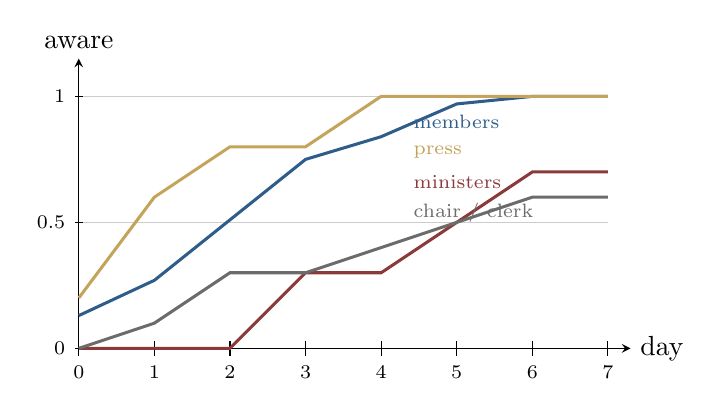
\begin{tikzpicture}[x=0.48cm,y=3.2cm]
  \draw[gray!40] (0,0.5) -- (14,0.5);
  \draw[gray!40] (0,1) -- (14,1);
  \draw[-stealth] (0,0) -- (14.6,0) node[right] {day};
  \draw[-stealth] (0,0) -- (0,1.15) node[above] {aware};
  \foreach \d in {0,1,2,3,4,5,6,7}
    \draw (\d*2,0.03) -- (\d*2,-0.03) node[below,font=\scriptsize] {\d};
  \foreach \y/\lab in {0/0, 0.5/0.5, 1/1}
    \draw (0.1,\y) -- (-0.1,\y) node[left,font=\scriptsize] {\lab};
  \draw[line width=1.1pt,color={rgb,255:red,47;green,93;blue,138}]
    (0,0.13) -- (2,0.27) -- (4,0.51) -- (6,0.75) -- (8,0.84) -- (10,0.97) -- (12,1.00) -- (14,1.00);
  \draw[line width=1.1pt,color={rgb,255:red,196;green,163;blue,90}]
    (0,0.20) -- (2,0.60) -- (4,0.80) -- (6,0.80) -- (8,1.00) -- (14,1.00);
  \draw[line width=1.1pt,color={rgb,255:red,139;green,58;blue,58}]
    (0,0.00) -- (2,0.00) -- (4,0.00) -- (6,0.30) -- (8,0.30) -- (10,0.50) -- (12,0.70) -- (14,0.70);
  \draw[line width=1.1pt,color={rgb,255:red,107;green,107;blue,107}]
    (0,0.00) -- (2,0.10) -- (4,0.30) -- (6,0.30) -- (8,0.40) -- (10,0.50) -- (12,0.60) -- (14,0.60);
  \node[font=\scriptsize,anchor=west,color={rgb,255:red,47;green,93;blue,138}] at (8.6,0.90) {members};
  \node[font=\scriptsize,anchor=west,color={rgb,255:red,196;green,163;blue,90}] at (8.6,0.78) {press};
  \node[font=\scriptsize,anchor=west,color={rgb,255:red,139;green,58;blue,58}] at (8.6,0.66) {ministers};
  \node[font=\scriptsize,anchor=west,color={rgb,255:red,107;green,107;blue,107}] at (8.6,0.54) {chair / clerk};
\end{tikzpicture}
\caption{Leak diffusion (S1, $N{=}25$, 5-seed mean). A resignation rumour
is seeded with one member in the wandelgang. Members reach $27\%$
awareness on day~1 and $\approx 100\%$ by day~7; the press is faster
($60\%$, then $100\%$), and ministers lag ($0\%$, then $70\%$). Only $4\%$
of Handelingen lines mention the leak.}
\label{fig:diffusion}
\end{figure}

\paragraph{Emergent behaviour.} A single seeded leak reached $27\%$ of
members and $60\%$ of the press within one day and essentially all members
and the press by day~7, whereas ministers remained unaware until day~3 and
reached $70\%$ by day~7 (Figure~\ref{fig:diffusion}). The same leak
appeared in only $4\%$ of simulated Handelingen lines
(Table~\ref{tab:interview}): members who knew it almost never put it on
the record, and journalists cannot speak on the floor. Rumour hops
embellished a detail $15\%$ of the time. Without the corridor network (GA
or --rumour), awareness stays at the seeded member ($5\%$).

\paragraph{Mechanisms.} The affordance layer is what makes the
Handelingen selective (Table~\ref{tab:interview}). Without it, as under
GA, every agent present at the sitting may speak: the official record grows
from $205$ to $4{,}876$ lines, and journalists occupy $4.3\%$ of it. No
role transitions occur in a one-week sitting, so --automaton matches the
full model on these metrics. The leak is carried by the rumour network,
not by the floor. Replacing the planner with \texttt{gpt-4o-mini} leaves
the selection diagnostics intact (Table~\ref{tab:backbone}): journalists
still occupy $0\%$ of the official record under standing orders and
$4.3\%$ without them, and the Handelingen still contain $205$ rather than
$4{,}876$ lines. The LLM does change behaviour: floor mention of the leak
rises from $4\%$ to $10\%$, and rumour hops embellish more often ($20\%$
vs.\ $15\%$). It cannot, however, put the press on the record or spread a
corridor leak unless the world allows it.

\begin{table}[t]
\caption{Selection-aware fidelity on held-out Tweede Kamer speeches
(1890--1899). Role JSD: lower is better. Journalist \% should be $0$.}
\label{tab:main}
\centering\small
\setlength{\tabcolsep}{4pt}
\begin{tabular}{lccc}
\toprule
Method & Role JSD $\downarrow$ & Journ.\ \% $\downarrow$ & Notes \\
\midrule
Archive (holdout) & --- & 0.0 & 20{,}166 speeches \\
Rule-ABM (1860--89 mix) & 0.001 & 0.0 & replay, no agents \\
GA~\cite{park2023generative} & 0.138 & 4.3 & ungated floor \\
\sys{} (naive calib.) & 0.129 & 2.2 & corridor counted \\
\sys{} (full) & 0.117 & \textbf{0.0} & 205 lines / week \\
\bottomrule
\end{tabular}
\end{table}

\paragraph{Macro fidelity.} The role mix is almost stationary between the
calibration and holdout decades (Rule-ABM JSD $0.001$), so simply
replaying the preceding thirty years matches \emph{who speaks}
(Table~\ref{tab:main}). The informative test is \emph{who must not
appear}. The archive never records a journalist; \sys{} reproduces that
zero, whereas GA and the affordance ablation do not. Naive calibration
(\S\ref{sec:calibration}) dilutes the official mix by treating wandelgang
talk as Handelingen and produces a $2.2\%$ press share that the archive
cannot contain. \sys{}'s role JSD ($0.117$) is higher than that of replay
because a 25-agent week over-represents the Chair relative to a full
chamber. This is a limit of scale; among the agent-based conditions,
\sys{} has the lowest role JSD (GA $0.138$, naive calibration $0.129$).

\begin{figure}[t]
\centering
\resizebox{\columnwidth}{!}{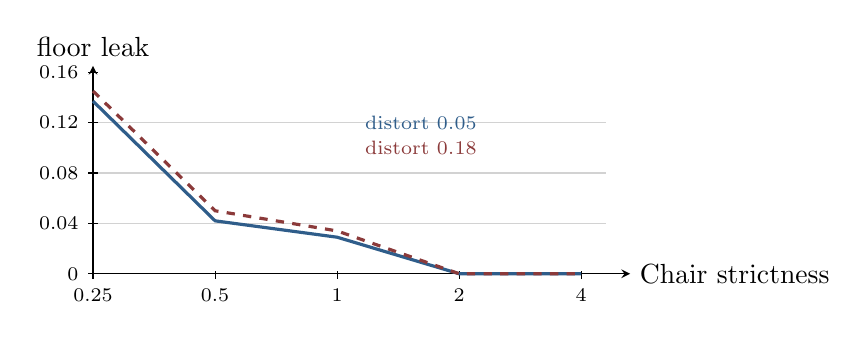
\begin{tikzpicture}[x=1.55cm,y=16cm]
  \draw[gray!35] (0,0.04) -- (4.2,0.04);
  \draw[gray!35] (0,0.08) -- (4.2,0.08);
  \draw[gray!35] (0,0.12) -- (4.2,0.12);
  \draw[-stealth] (0,0) -- (4.4,0) node[right] {Chair strictness};
  \draw[-stealth] (0,0) -- (0,0.165) node[above] {floor leak};
  \foreach \x/\lab in {0/0.25, 1/0.5, 2/1, 3/2, 4/4}
    \draw (\x,0.002) -- (\x,-0.004) node[below,font=\scriptsize] {\lab};
  \foreach \y/\lab in {0/0, 0.04/0.04, 0.08/0.08, 0.12/0.12, 0.16/0.16}
    \draw (0.04,\y) -- (-0.04,\y) node[left,font=\scriptsize] {\lab};
  \draw[line width=1.15pt,color={rgb,255:red,47;green,93;blue,138}]
    (0,0.137) -- (1,0.042) -- (2,0.029) -- (3,0.000) -- (4,0.000);
  \draw[line width=1.15pt,dashed,color={rgb,255:red,139;green,58;blue,58}]
    (0,0.145) -- (1,0.050) -- (2,0.034) -- (3,0.000) -- (4,0.000);
  \node[font=\scriptsize,anchor=west,color={rgb,255:red,47;green,93;blue,138}] at (2.15,0.12) {distort $0.05$};
  \node[font=\scriptsize,anchor=west,color={rgb,255:red,139;green,58;blue,58}] at (2.15,0.10) {distort $0.18$};
\end{tikzpicture}}
\caption{S3 intervention (3-seed mean). Raising Chair strictness drives
the leak off the official record; corridor distortion changes the rate
only while the Chair still grants the floor.}
\label{fig:cf}
\end{figure}

\paragraph{Interventions.} Floor mention falls from $14\%$ at
$0.25\times$ Chair strictness to $3\%$ at the default and to $0$ at
$2\times$ and above (Figure~\ref{fig:cf}). Distortion ($0.05$ vs.\
$0.18$) shifts the rate by about one percentage point while recognition is
frequent, and not at all once the Chair stops granting the floor. These
are model-internal counterfactuals. They show that, within \sys{}, what
reaches the record can be controlled through the procedural parameters of
the world without changing the agents' cognitive backend.

\paragraph{Audit.} Modern-vocabulary hits in official lines are $0\%$ on
both the heuristic backend and \texttt{gpt-4o-mini}. Full \sys{} writes
structured refusals for unrecognised members and the journalist ($22$ of
$25$ agents in the heuristic week and in LLM seed~7); GA writes none on
either backbone. Procedure, not prompt wording, keeps the press off the
record. This inverts the situation in Smallville, where the language model
made agents overly cooperative~\cite{park2023generative}; in \sys{}, the
world's procedure decides who may speak.

\begin{table}[t]
\caption{TrueSkill ranking of pause-and-interview answers by one historian
(\sys{} with LLM vs.\ Smallville-style GA). Attention checks passed: $2/2$.
Higher $\mu$ is better; $\sigma$ is the posterior uncertainty.}
\label{tab:historian}
\centering\small
\setlength{\tabcolsep}{3.5pt}
\begin{tabular}{lcccc}
\toprule
Condition & $\mu_{\text{bel}}$ & $\sigma$ & $\mu_{\text{proc}}$ & $\sigma$ \\
\midrule
\sys{} (full, LLM) & \textbf{28.3} & 1.8 & \textbf{27.8} & 2.2 \\
GA~\cite{park2023generative} & 21.7 & 1.8 & 22.2 & 2.2 \\
\bottomrule
\end{tabular}\\[4pt]
{\raggedright\scriptsize Pairwise (full vs.\ GA): believability 17--8--11
(win--loss--tie); procedure 12--5--19. One pair was left unranked with a
written comment (``Kamerlid der Tweede/Eerste Kamer'', not ``MP'').\par}
\end{table}

\paragraph{Historian review.} The rater passed both attention checks,
which planted obvious anachronisms (a Twitter livestream; ``I am a large
language model''). On the remaining pairs, \sys{} outranked the
Smallville-style ablation on both criteria (Table~\ref{tab:historian}).
Ties were more frequent for procedure than for believability, consistent
with both systems being prompted about recognition. The standing-order
vignettes matched the intended $\pi$: a journalist on the floor is out of
order and off the record, as is an unrecognised interruption, whereas
wandelgang talk is in order but not part of the Handelingen. The rater
asked us to separate the griffier from the stenographer, to let Kamerleden
speak in afdeelingen without plenary recognition, to let ministers talk in
the wandelgang, and, in the comment that most changed the world, to stop
treating the Tweede and Eerste Kamer as one chamber. On the OCR speaker
cards, $27/40$ names were accepted, with a mean OCR quality of $3.8/5$.
Party was the weakest field ($18$ yes / $13$ no / $7$ uncertain) because
1890s ``parties'' were kamerclubs (parliamentary factions) that could
merge, as the Bahlmannianen and Schaepmannianen did into a Roman Catholic
bloc in 1896. Following this review, S1 seeds the Pierson cabinet in office
at $t_0$ (Cremer at Colonies, Goeman Borgesius at Interior, Gleichman in
the chair, Arntzenius as griffier) and drops van Houten, Sprenger van Eyk,
and Gerritsen, who did not hold those posts in December 1899. The
heuristic leak results (Table~\ref{tab:interview}) predate this roster
correction; minister identity does not change who may speak.

\paragraph{Simulated vs.\ real silence.} In Figure~\ref{fig:teaser}, the
Handelingen page records a recognised speech on the East Indies budget,
while the resignation leak, the journalist's notes, and the minister who
has not yet heard of it remain invisible to the stenographer. The
simulated Handelingen thus reproduces the structural silences of the real
one~\cite{trouillot1995silencing}, and the sandbox makes the gap between
them inspectable.

%% =====================================================================
\section{Discussion}
\label{sec:discussion}

\paragraph{What a sandbox can claim.} \sys{} produces \emph{sufficiency}
evidence: mechanisms that, under explicit assumptions, generate patterns
consistent with the Handelingen. It cannot establish what any historical
member thought; agents' reflections are model artefacts, not recovered
voices. The sandbox is valuable because it makes historians' assumptions
about procedure and selection explicit and manipulable, and because it
generates hypotheses for further archival work in committee minutes,
private correspondence, and the press.

\paragraph{Interactivity as method.} Inspection, interviews, and object
edits are the intended way for historians to find errors in the
standing-order rules. The ablations isolate those rules with a heuristic
planner, and the backbone check (Table~\ref{tab:backbone}) shows the same
selection pattern under \texttt{gpt-4o-mini}. The historian ranking
(Table~\ref{tab:historian}) is a first measurement of believability; it
complements the selection test rather than replacing it.

\paragraph{Limitations.} The 1814--1899 slice is OCR-noisy, speaker
strings do not identify unique persons, and 1890s party labels denote
kamerclubs rather than mass parties. The Binnenhof is a composite, and the
journalist is a synthetic observer. S1 is a 25-agent Tweede Kamer week, so
it cannot match the role mix of a full chamber, and it runs no Eerste Kamer
sitting even though senate tiles and affordances exist in the world. S3
does not simulate the 1848 constitutional revision, and a single historian
ranked the interviews. We release seeds, configurations, and the DutchParl
parser.

%% =====================================================================
\section{Ethical Considerations}
\label{sec:ethics}

\paragraph{Why not a slave-society sandbox.} An earlier version of this
project proposed generative agents of a colonial Caribbean slave society,
calibrated to newspapers that printed runaway advertisements. Historians we
consulted objected that simulating enslaved people, even as synthetic
personas and even under institutional constraints, risks reproducing the
dehumanisation of the archive, trivialising violence, and presenting
fabrication as recovered
experience~\cite{hartman2008venus,fuentes2016dispossessed}. We agreed and
abandoned that design. \sys{} instantiates no enslaved, colonised, or
otherwise unfree persons as agents. Colonial policy appears only as it
appears in the Handelingen: as speech by metropolitan office-holders,
which the sandbox may reproduce as public speech but never as the inner
life of the people discussed.

\paragraph{Commitments for a parliamentary sandbox.}
(1)~\emph{Public persons in public roles.} Agents are seeded from
attested speakers in CC0 proceedings; we do not invent private lives,
families, or unrecorded interiors.
(2)~\emph{No gamification.} There is no playable persona, no score, and
no first-person control of the Chair or of ministers.
(3)~\emph{Provenance.} All simulated text, including the simulated
Handelingen, is labelled and kept separate from the archival XML.
(4)~\emph{Procedure over psychology.} Claims concern standing orders,
selection, and diffusion, not what a named member ``really thought''.
(5)~\emph{Consultation.} The project is designed with historians of
Dutch politics. The labelling reported here was carried out with informed,
task-specific consent, and the rater could skip any item.
(6)~\emph{Copyright.} The source corpus is released under CC0, and
Auteurswet art.~11 places official proceedings outside copyright. We cite
Marx et al.~\cite{marx2012dutchparl} as the source of the corpus.

%% =====================================================================
\section{Conclusion}
\label{sec:conclusion}

We presented \sys{}, an interactive generative agent sandbox of Dutch
parliamentary debate in which roles, standing orders, corridor talk, and
the selection process that produces the Handelingen are explicit parts of
the world. \sys{} replaces Smallville's open town with a Binnenhof where
every speech on the floor must be recognised, and it writes its own
proceedings. In a one-week sitting, a leak known to almost all members
appeared in only $4\%$ of official lines, and journalists stayed out of
the record under both the heuristic planner and \texttt{gpt-4o-mini}.
Procedure alone was enough to separate what parliament knew from what its
record says. Silence in the Handelingen therefore cannot by itself be read
as ignorance, and simulations of archived institutions should be
calibrated on what their own stenographers record. Used in this way,
generative agents become instruments for generating historical hypotheses,
without asking a language model to stand in for people whom the archive
has already silenced.

%% =====================================================================
\begin{acks}
Anonymised for review.
\end{acks}

\bibliographystyle{ACM-Reference-Format}
\bibliography{references}

\end{document}
